\documentclass[a4paper,11pt,exos]{nsi} % COMPILE WITH DRAFT
\usepackage{pifont}
\usepackage{fontawesome5}
\usepackage{hyperref}

\usepackage{pgfplots}

\pgfplotsset{compat=newest}
\pgfplotsset{every axis/.append style={
                    axis x line=middle,
                    axis y line=middle,
                    axis line style={->},
                    xlabel={$x$},
                    ylabel={$y$},
                    label style={font=\scriptsize},
                    tick label style={font=\tiny},
                    unit vector ratio*=1 1 1,
   					xlabel style={at={(ticklabel* cs:1)},anchor=north west},
   					ylabel style={at={(ticklabel* cs:1)},anchor=south west}
                    }}

\begin{document}
\classe{\premiere spé}
\titre{Fonction exponentielle}
\maketitle

\setlength{\columnseprule}{0pt}
\setlength{\columnsep}{30pt}


On souhaite construire de  de façon approchée la courbe représentative d'une fonction dérivable $f$ qui vérifie
$$f '(a)=f (a) \text{ pour tout réel } a\quad \text{et} \quad f(0)=1 .$$
Nous allons utiliser la méthode d’Euler qui repose sur l'utilisation d'une
approximation affine d'une fonction en un point et donc construire point par point $\mathcal{C}_f$, la courbe représentative de $f$.

\begin{center}
    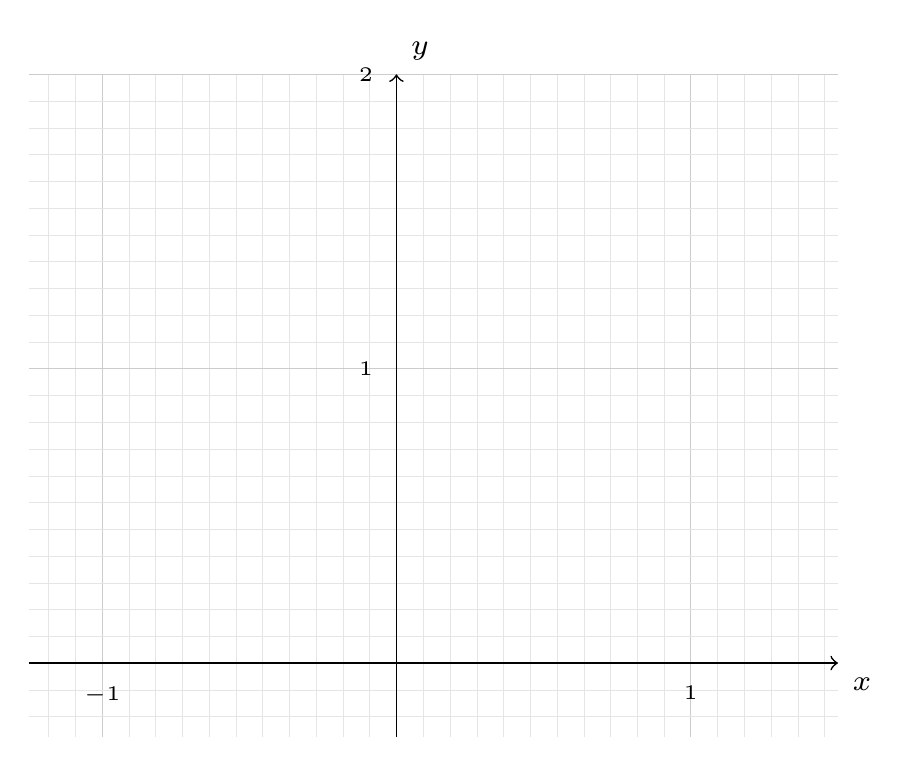
\begin{tikzpicture}[scale=1.5]
        \begin{axis}[
            name = graph1,
            ytick distance = 1,
            xtick distance = 1,
            ymin=-.25, ymax=2,
            xmin=-1.25, xmax=1.5,
            grid=both,
            grid style={line width=.1pt,draw=gray!20},
            major grid style={line width=.2pt,draw=gray!40},
            minor tick num=10,
            tick style={draw=none},
          ]
       
            %\draw[thick,UGLiBlue,domain=0:0.35,smooth,variable=\x] plot ({\x},{.9*\x*(1-\x)});
            %\draw[thick,UGLiRed,domain=0:0.35,smooth,variable=\x] plot ({\x},{\x});
            %\draw[UGLiBlue] (0.33,.2) node[above]{$\mathcal{C}_f$}  ;
            %\draw[UGLiRed] (0.25,.25) node[below]{$d$}  ;
          \end{axis}
    \end{tikzpicture}
\end{center}


\subsection*{Étape 1 : $f(0)=1$}
On a donc $f'(0)=..........$\\
Placer $A$ le premier point de $\mathcal{C}_f$ et tracer $T_A$ la tangente à $\mathcal{C}_f$ en ce point.

\subsection*{Étape 2 : Approximation de $f(0,1)$}
\dleft{10.5cm}{
    Sur la figure ci-contre, $B$ est le point de $\mathcal{C}_f$ d’abscisse $0,1$.\\
    Comme $B$ est proche de $A$, la droite $(AB)$ est proche de la tangente à $\mathcal{C}_f$ en $A$. Donc le coefficient directeur de la droite $(AB)$, $\dfrac{f(0,1)-f(0)}{0,1-0}$ est proche du coefficient directeur de $(T_A)$ égal à $f'(0)$.\\
    Donc $\quad \dfrac{f(0,1)-f(0)}{0,1-0}\approx f'(0)$.\\
    
}
{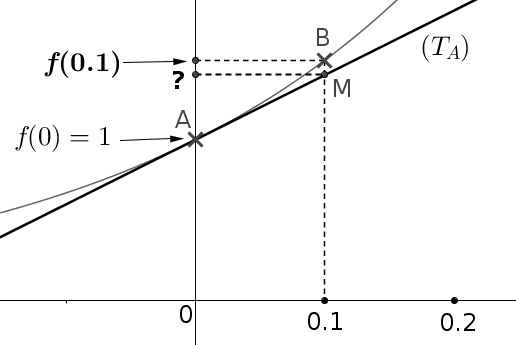
\includegraphics[width=6cm]{courbe1.png}}
En utilisant cette approximation, donner une approximation de $f(0,1)$ et placer le point $B$ correspondant.

\dleft{10.5cm}{
    \subsection*{Étape 3 : Approximation de $f(0,2)$}
    Comme précedemment $\quad \dfrac{f(0,2)-f(0,1)}{0,2-0,1}\approx f'(0,1)$.\\

    En déduire une approximation de $f(0,2)$ et placer le point $C$ correspondant.
}
{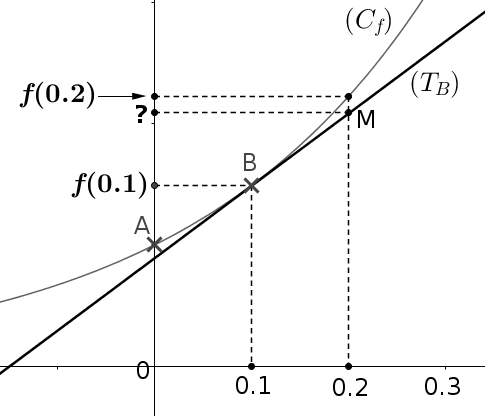
\includegraphics[width=6cm]{courbe2.png}}

\subsection*{Étape 4}
Compléter le tableau suivant. Si besoin, effectuer au brouillon les calculs pour les trois dernières colonnes ou mettre en évidence un moyen rapide de calculer les approximations demandées.\\

\tabstyle[UGLiOrange]
\begin{tabular}{|c|c|c|c|c|c|c|}
\hline
\ccell $x$ & $0$ & $0,1$ & $0,2$ & $0,3$ & $0,4$ & $0,5$ \\\hline
\ccell Approximation de $f(x)$ & $1$ & \hspace*{1.5cm} & \hspace*{1.5cm} & \hspace*{1.5cm} & \hspace*{1.5cm} & \hspace*{1.5cm}  \\\hline
\end{tabular}
\end{document}